\begin{corollary}
	In any HTS, if \(\mc{K}\) is compact, and \(\mc{F}\) is closed, then \(\mc{K}\cap\mc{F}\) is compact.
\end{corollary}
\begin{proof}
	\(\mc{K}\cap\mc{F}\) is closed, and \(\mc{K}\cap\mc{F}\subseteq\mc{K}\).
\end{proof}

\begin{corollary}
	Let \(\mc{K}\) be compact in some HTS, any infinite set \(\mc{A}\subseteq\mc{K}\) must have \(\mc{A}'\neq\emptyset\).
\end{corollary}
\begin{proof}
	By prove this by contrapositive. Suppose \(\mc{S}\subseteq\mc{K}\) has \(\mc{S}'=\emptyset\). For each \(x\in\mc{S}\), \(x\notin\mc{S}'\), which implies some open \(\mc{G}_x\) obeys \(\mc{G}_x\cap\mc{S}=\{x\}\). Thus, \(\ms{G}=\{\mc{G}_x:x\in\mc{S}\}\) is an open cover for \(\mc{S}\). Observe that \(\ol{\mc{S}}=\mc{S}\cup\mc{S}'=\mc{S}\) is closed, so it is compact; hence \(\ms{G}\) has a finite subcover \(\mc{G}_{x_1},\mc{G}_{x_2},\dots,\mc{G}_{x_N}\), i.e., \(\mc{S}\subseteq\mc{G}_{x_1}\cup\mc{G}_{x_2}\cup\dots\cup\mc{G}_{x_N}\). Therefore, by construction, \(\mc{S}=\{x_1,x_2,\dots,x_N\}\) is finite.
\end{proof}

\subsubsection{Complementary view of compactness}
\begin{ndef}{: Finite intersection property}
	A family of sets \(\ms{F}\) has the \emph{\textbf{finite intersection property}} (F.I.P.) if every finite choice of \(\mc{F}_1,\mc{F}_2,\dots,\mc{F}_N\in\ms{F}\) gives \(\displaystyle\bigcap_{k=1}^N \mc{F}_k\neq\emptyset\).
\end{ndef}

\begin{ntheorem}{}
	In any HTS \((\mc{X},\ms{T})\) with subset \(\mc{K}\subseteq\mc{X}\), assume \(\mc{K}\) is closed. Then, the following are equivalent:
	\begin{enumerate}[(a)]
		\item \(\mc{K}\) is compact.
		
		\item Every family \(\ms{F}\) of \emph{closed} subsets of \(\mc{K}\) with F.I.P. has \(\displaystyle\bigcap\ms{F}\neq\emptyset\).
	\end{enumerate}
\end{ntheorem}
\begin{proof}[Proof sketch]
	Left as practice (advised to do proof by contrapositive).
\end{proof}

\subsection{Convergence}
\begin{ntheorem}{}
	In a metric space \((\mc{X}, d)\) with \(\mc{K}\subseteq\mc{X}\), the following are equivalent:
	\begin{enumerate}[(a)]
		\item \(\mc{K}\) is compact.
		
		\item Every sequence \((x_n)\) in \(\mc{K}\) has a subsequence that converges to a point in \(\mc{K}\).
	\end{enumerate}
\end{ntheorem}

\begin{proof}
	\((a\Rightarrow b)\) Let \((x_n)\) be a sequence in \(\mc{K}\). Consider \(\mc{A}=\{x_n:n\in\N\}\) be the range of that sequence. If \(\mc{A}\) is finite, a constant subsequence exists (some point of \(\mc{A}\) is ``hit" by infinitely many \(x_n\)). Otherwise, \(\mc{A}'\neq\emptyset\); any \(x\in\mc{A}'\) will have \(\mc{A}\cap\B\left(x;\displaystyle\frac{1}{n}\right)\neq\emptyset\). Standard methods will give subsequence of \((x_n)\) converging to \(x\). Furthermore, \(x\in\mc{A}'\subseteq\mc{K}\) because \(\mc{K}\) is closed.
	
	\medskip
	
	\((b\Rightarrow a)\) Let \(\mc{K}\) have property in (b). Given arbitrary open cover \(\ms{G}\) for \(\mc{K}\), for each \(x\in\mc{K}\), some \(\mc{G}\subseteq\ms{G}\) obeys \(x\in\mc{G}\). Consider 
	\begin{equation*}
		R(x)=\begin{cases}
					\sup\{\eps>0:\B[x;\eps)\subseteq\mc{G}\},~\text{for some}~\mc{G}\in\ms{G},&\text{if the RHS is not}~+\infty.\\
					
					1,&\text{otherwise}.
				  \end{cases}
	\end{equation*}
	Then, let \(r(x)=\displaystyle\frac{1}{2}R(x)\); for all \(x\in\mc{K}\), \(\B[x;r(x))\subseteq\mc{G}\) holds for some \(\mc{G}\in\ms{G}\).
	
	\medskip
	
	\begin{align*}
		&\text{Pick any}~x_1\in\mc{K};~\text{write}~r_1=r(x_1).\\
		&\text{Pick any}~x_2\in\mc{K}\backslash\B[x_1;r_1)~\text{write}~r_2=r(x_2).\\
		&\text{Pick any}~x_3\in\mc{K}\backslash\B[x_1;r_1)\cup\B[x_2;r_2));~\text{write}~r_3=r(x_3)\\
		&\vdots
	\end{align*}
	Expect a sequence of \(x_1,x_2,\dots\) with corresponding \(r_1,r_2,r_3,\dots\) such that if \(q>p\), \(x_q\notin\B[x_p;r_p)\), i.e., \(d(x_q,x_p)\geq r_p\).
	\begin{claim}
		This construction \emph{cannot} run forever.
	\end{claim}
	\begin{proof}
		For the sake of contradiction, suppose this does work and produce a sequence \((x_n)\) in \(\mc{K}\). Use (b) to get a subsequence \((x_{n_k})\) and \(\hat{x}\in\mc{K}\) such that \(x_{n_k}\to\hat{x}\) as \(k\to\infty\). Note that \((p=n_k,~q=n_{k+1}~\text{above})\)
		\begin{align*}
			r_{n_k}\leq&d(x_{n_{k+1}},x_{n_{k}})\\
				   \leq&d(x_{n_{k+1}},\hat{x})+d(\hat{x},x_{n_k})\to 0+0~\text{as}~k\to\infty,
		\end{align*}
		so \(r_{n_k}\to 0\). Now, \(\hat{x}\in\mc{K}\), so \(r(\hat{x})\) is defined and \(\B[\hat{x};r(\hat{x}))\subseteq\hat{\mc{G}}\) for some \(\hat{\mc{G}}\subseteq\ms{G}\). Use \(x_{n_k}\to\hat{x}\) to say that for all sufficiently large \(k\), \(d(x_{n_k},\hat{x})<\displaystyle\frac{1}{2}r(\hat{x})\). So, 
		\begin{equation*}
			\B\left[x_{n_k};\frac{r(\hat{x})}{2}\right)\subseteq \B\left[\hat{x};r(\hat{x})\right)\subseteq\hat{\mc{G}},
		\end{equation*} 
		and hence \(R(x_{n_k})\geq\displaystyle\frac{1}{2}r(\hat{x})\), so 
		\begin{equation*}
			r_{n_k}=\frac{1}{2}R(x_{n_k})\geq\frac{1}{4}r(\hat{x}),
		\end{equation*}
		which is a contradiction. So construction must fail at some stage. Therefore,
		\begin{equation*}
			\mc{K}\backslash\left(\B[x_1;r_1)\cup\B[x_2;r_2)\cup\dots\cup\B[x_M;r_M)\right)=\emptyset,
		\end{equation*} 
		or
		\begin{equation*}
			\mc{K}\subseteq\B[x_1;r_1)\cup\dots\cup\B[x_M;r_M).
		\end{equation*}
		Each of these balls fits inside some corresponding \(\mc{G}_k\) from \(\ms{G}\); finite subcover has been found.
	\end{proof}
	\begin{figure}[htbp]
		\centering
		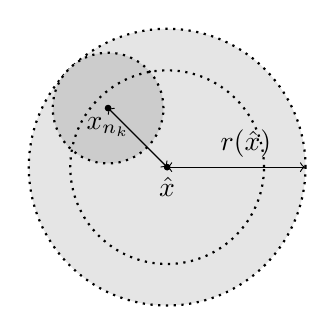
\begin{tikzpicture}
			\draw[black, dotted, thick, fill = white!60!lightgray] (0,0) circle (50pt);
			\draw[fill] (0,0) circle (1pt);
			\node[below] at (0,0) {\(\hat{x}\)};
			\draw[black, dotted, thick, fill = white!60!gray] (-0.75,0.75) circle (20pt);
			\draw[fill] (-0.75,0.75) circle (1pt);
			\node[below] at (-0.75,0.75) {\(x_{n_k}\)};
			\draw[black, dotted, thick] (0,0) circle (35pt);
			\draw[<->] (-0.75,0.75) -- (0,0);
			\draw[<->] (0,0) -- (1.75,0);
			\node[above] at (1,0) {\(r(\hat{x})\)};
		\end{tikzpicture}
		\caption{Visualization of the construction in the proof.}
	\end{figure}
\end{proof}